% Copyright 2004 by Till Tantau <tantau@users.sourceforge.net>.
%
% In principle, this file can be redistributed and/or modified under
% the terms of the GNU Public License, version 2.
%
% However, this file is supposed to be a template to be modified
% for your own needs. For this reason, if you use this file as a
% template and not specifically distribute it as part of a another
% package/program, I grant the extra permission to freely copy and
% modify this file as you see fit and even to delete this copyright
% notice. 

\documentclass{beamer}
% Replace the \documentclass declaration above
% with the following two lines to typeset your 
% lecture notes as a handout:
%\documentclass{article}
%\usepackage{beamerarticle}

\usepackage{graphicx}
\usepackage[utf8]{inputenc}
\usepackage{tabto}
 
\graphicspath{ {img/} }


% There are many different themes available for Beamer. A comprehensive
% list with examples is given here:
% http://deic.uab.es/~iblanes/beamer_gallery/index_by_theme.html
% You can uncomment the themes below if you would like to use a different
% one:
%\usetheme{AnnArbor}
%\usetheme{Antibes}
%\usetheme{Bergen}
%\usetheme{Berkeley}
%\usetheme{Berlin}
%\usetheme{Boadilla}
%\usetheme{boxes}
%\usetheme{CambridgeUS}
%\usetheme{Copenhagen}
%\usetheme{Darmstadt}
%\usetheme{default}
%\usetheme{Frankfurt}
%\usetheme{Goettingen}
%\usetheme{Hannover}
%\usetheme{Ilmenau}
%\usetheme{JuanLesPins}
%\usetheme{Luebeck}
%\usetheme{Madrid}
%\usetheme{Malmoe}
%\usetheme{Marburg}
%\usetheme{Montpellier}
%\usetheme{PaloAlto}
%\usetheme{Pittsburgh}
%\usetheme{Rochester}
%\usetheme{Singapore}
%\usetheme{Szeged}
\usetheme{Warsaw}

\title{Programming with Python}

% A subtitle is optional and this may be deleted
\subtitle{Lesson 5: Dictionaries and Tuples!}

%\author{F.~Author\inst{1} \and S.~Another\inst{2}}
% - Give the names in the same order as the appear in the paper.
% - Use the \inst{?} command only if the authors have different
%   affiliation.

%\institute[Universities of Somewhere and Elsewhere] % (optional, but mostly needed)
%{
%  \inst{1}%
%  Department of Computer Science\\
%  University of Somewhere
%  \and
%  \inst{2}%
%  Department of Theoretical Philosophy\\
%  University of Elsewhere}
% - Use the \inst command only if there are several affiliations.
% - Keep it simple, no one is interested in your street address.

\date{November 29th, 2016}
% - Either use conference name or its abbreviation.
% - Not really informative to the audience, more for people (including
%   yourself) who are reading the slides online

\subject{Python Lessons}
% This is only inserted into the PDF information catalog. Can be left
% out. 

% If you have a file called "university-logo-filename.xxx", where xxx
% is a graphic format that can be processed by latex or pdflatex,
% resp., then you can add a logo as follows:

% \pgfdeclareimage[height=0.5cm]{university-logo}{university-logo-filename}
% \logo{\pgfuseimage{university-logo}}

% Delete this, if you do not want the table of contents to pop up at
% the beginning of each subsection:
%\AtBeginSubsection[]
%{
%  \begin{frame}<beamer>{Outline}
%    \tableofcontents[currentsection,currentsubsection]
%  \end{frame}
%}

% Let's get started
\begin{document}

\begin{frame}
  \titlepage
\end{frame}

%\begin{frame}{Outline}
%  \tableofcontents
%  % You might wish to add the option [pausesections]
%\end{frame}

% Section and subsections will appear in the presentation overview
% and table of contents.
\section{Introduction \& Recap}

\begin{frame}{Last week's goals}
\pause
  \begin{itemize}
  \item We learnt about lists\pause
  \item We learnt about how we can iterate on lists with a for loop\pause
  \item We learnt about some list operations\pause
  \item We begun writing our own text based game!
  \end{itemize}
  
\end{frame}

\section{Tuples}

\begin{frame}{A flashback to lists}

Lists - A collection of anything you want\\ \pause

Can be resized\\ \pause

Elements can be changed when we want

\end{frame}

\begin{frame}{Tuples}

Tuples - A collection of anything you want\\ \pause

Cannot be resized\\ \pause

Once made, elements cannot be changed - You will not be able to do for example x[0] = 4. \pause This means tuples are \textit{immutable}.

\end{frame}

\begin{frame}{Tuple syntax}

\begin{figure}[h]
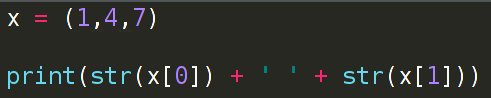
\includegraphics[width=0.8\textwidth]{tuple}
\end{figure}
\pause
\begin{figure}[h]
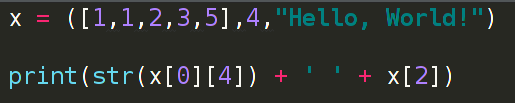
\includegraphics[width=0.8\textwidth]{tuple2}
\end{figure}


\end{frame}


\begin{frame}{What's the point?}

As tuples are immutable, they are much faster.\\ \pause

We can also use tuples if we want to return multiple values from a function.

\end{frame}

\begin{frame}{Example involving functions}

\begin{figure}[h]
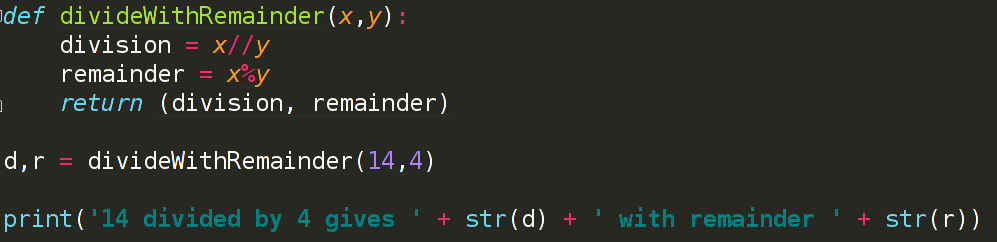
\includegraphics[width=0.99\textwidth]{tuplefunc}
\end{figure}
\pause
Note the neat syntax on the left of the equals sign. You can kind of 'map' variables to the locations in a tuple.
\end{frame}

\section{Dictionaries}

\begin{frame}{What is a dictionary}

Dictionaries are big 'lists' of key-value pairs.\\ \pause
Keys can be ints, floats, strings, or tuples. Values can be absolutely anything.\\ \pause
They have plenty of uses, including:

  \begin{itemize}
  \item Storing place name to coordinates for a GPS tracking app\pause
  \item Storing weapon names to weapon stats for a game\pause
  \item Translating something from english to german
  \end{itemize}

\end{frame}

\begin{frame}{An example of a dictionary}

\begin{figure}[h]
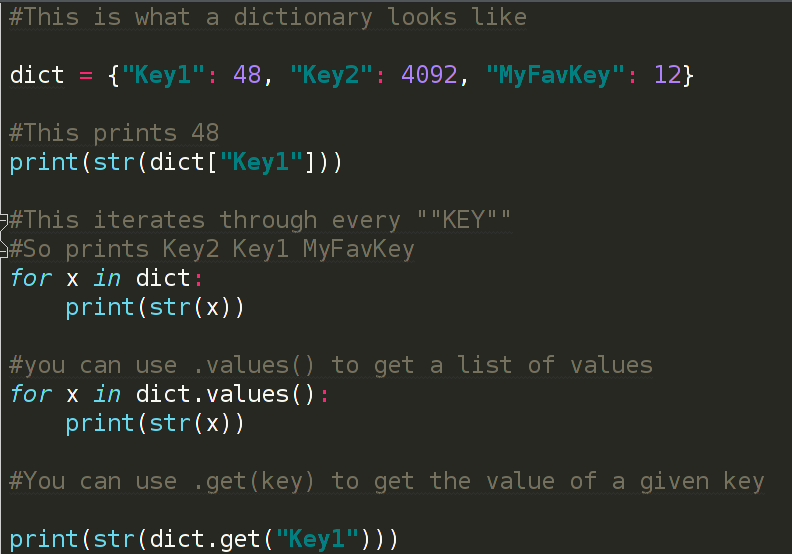
\includegraphics[width=0.85\textwidth]{dict}
\end{figure}

\end{frame}

\section{Objects \& Classes}

\begin{frame}{Objects \& classes}

Objects are ways to store more advanced structures of data\\ \pause

An object is a physical version of a class - like if an object were a car, it's class would be it's blueprints\\ \pause

There's a tonne of stuff on objects and classes online, though they are not for the faint of heart!

\end{frame}

\section{More Games}

\begin{frame}
Time for more games!
\end{frame}

\begin{frame}{presentations!}

\end{frame}

\section{Summary}

\begin{frame}{That's all for tonight}
  To summarise:
  \pause
  \begin{itemize}
  \item We learnt about tuples and their uses in returning multiple values\pause
  \item We learnt about dictionaries\pause
  \item We discussed objects\pause
  \item We finished writing our own text based game!
  \end{itemize}
\end{frame}

\begin{frame}{For next week}
Source code plus lecture slides will be available online soon after the lesson.\\
If you are new to HackSocNotts, please join us on \textit{http://hacksocnotts.slack.com}.\\
If you have any questions, feel free to ask now or over slack.\\
\end{frame}

\end{document}


